


\begin{figure}[tbp]
  \begin{center}
        \subfloat[line]{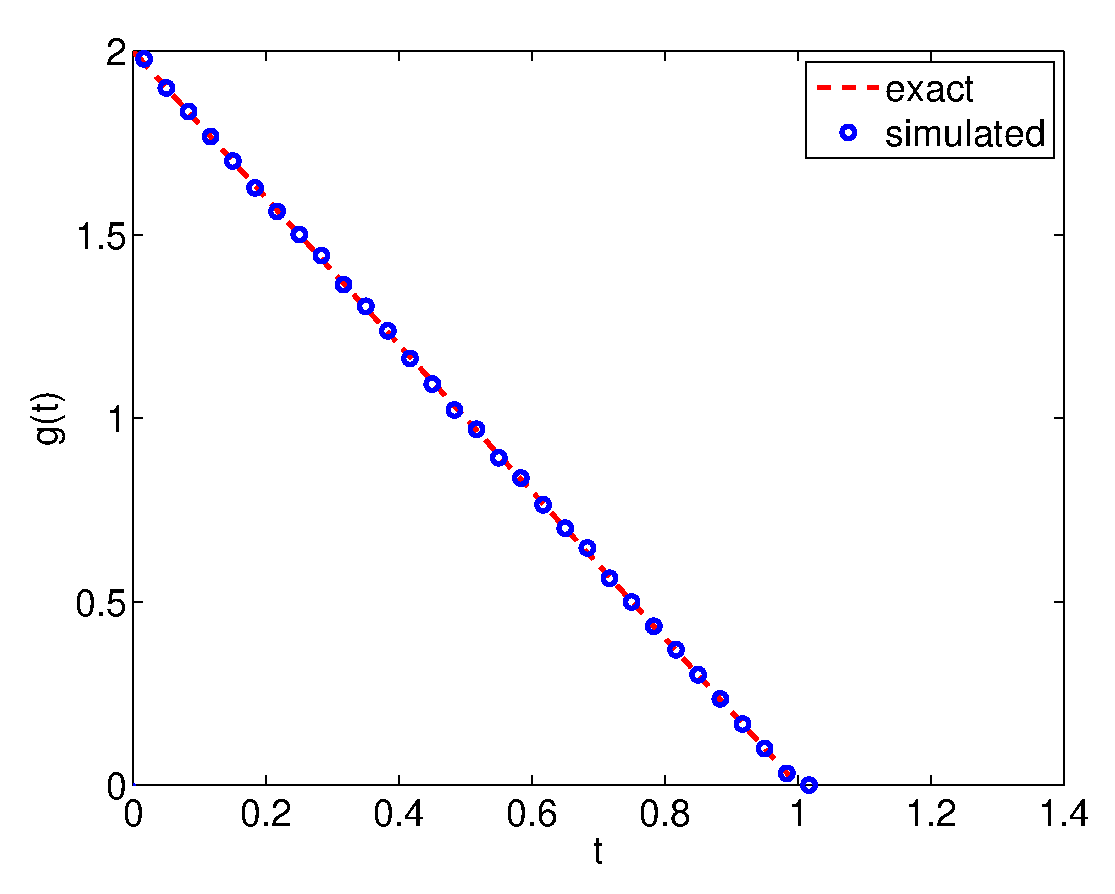
\includegraphics[width=0.24\columnwidth]{../Matlab/Plots/LinePicking_test_sim_line.eps}}
        \subfloat[square]{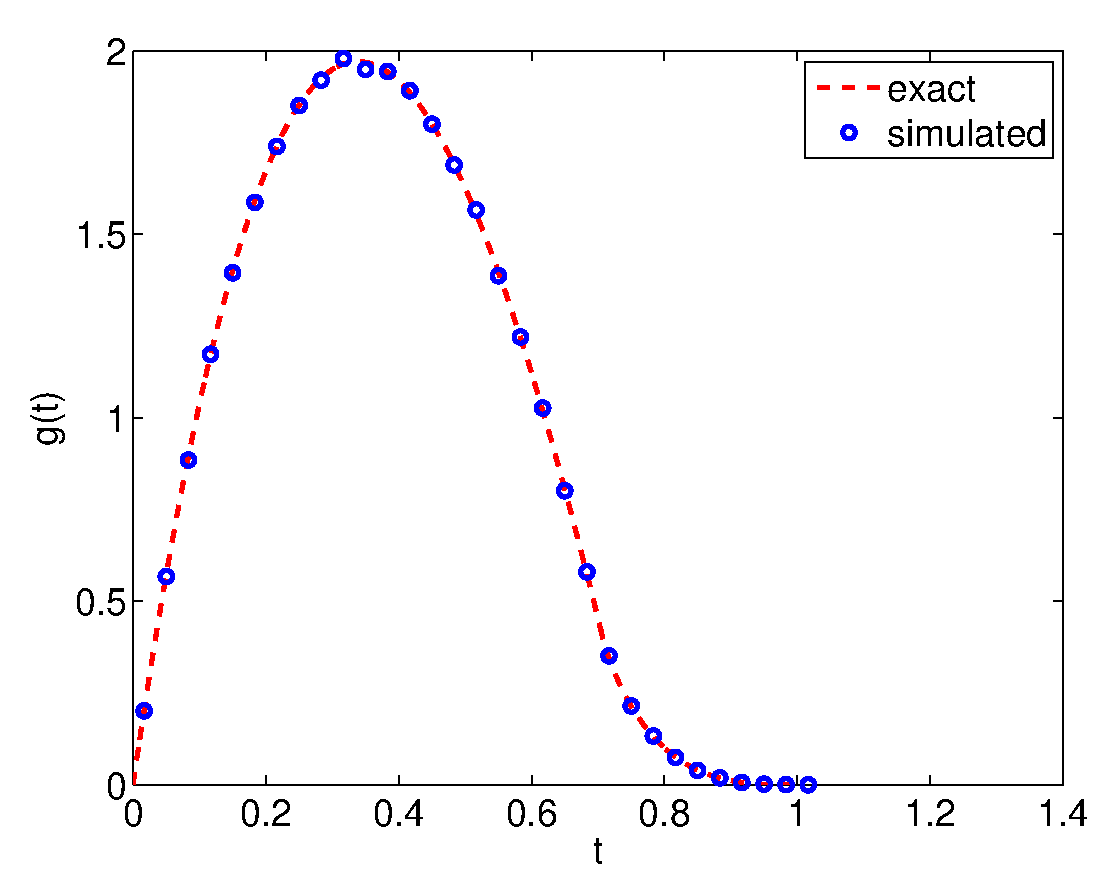
\includegraphics[width=0.24\columnwidth]{../Matlab/Plots/LinePicking_test_sim_square.eps}}
        \subfloat[cube]{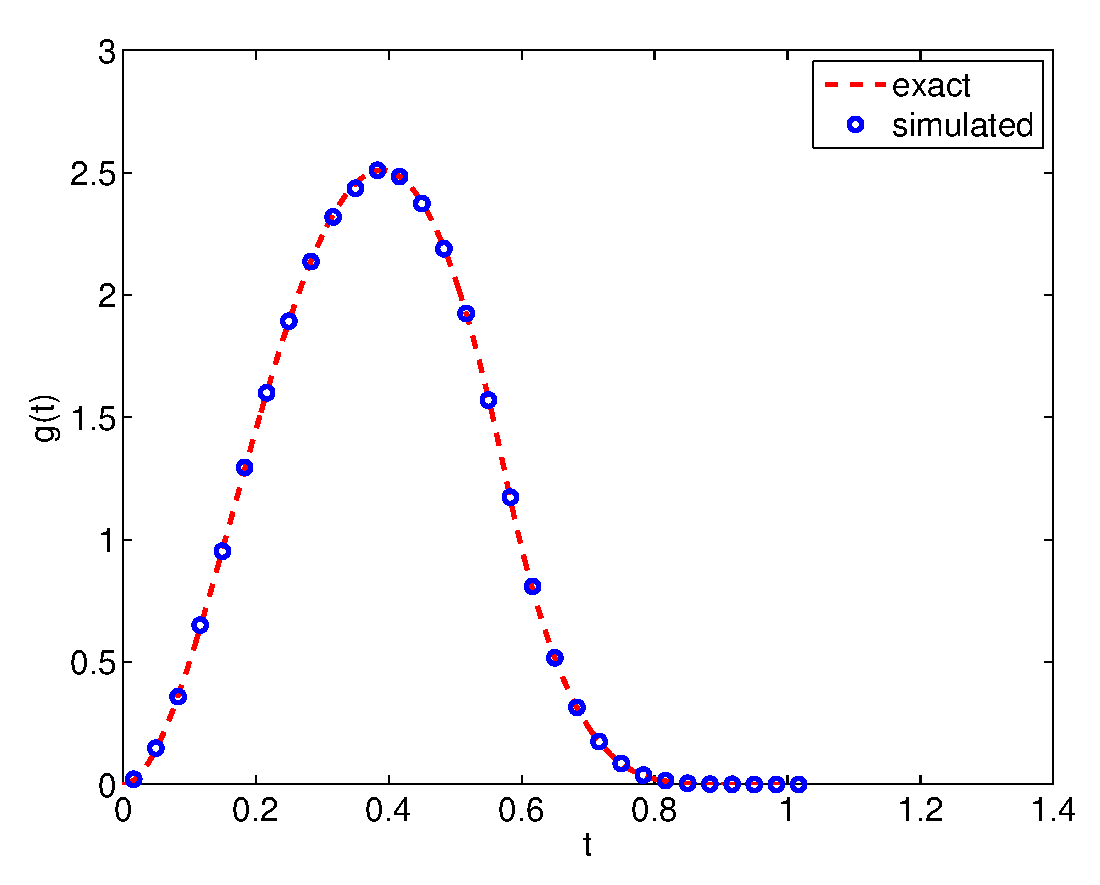
\includegraphics[width=0.24\columnwidth]{../Matlab/Plots/LinePicking_test_sim_cube.eps}}
        \subfloat[rectangle (1:2)]{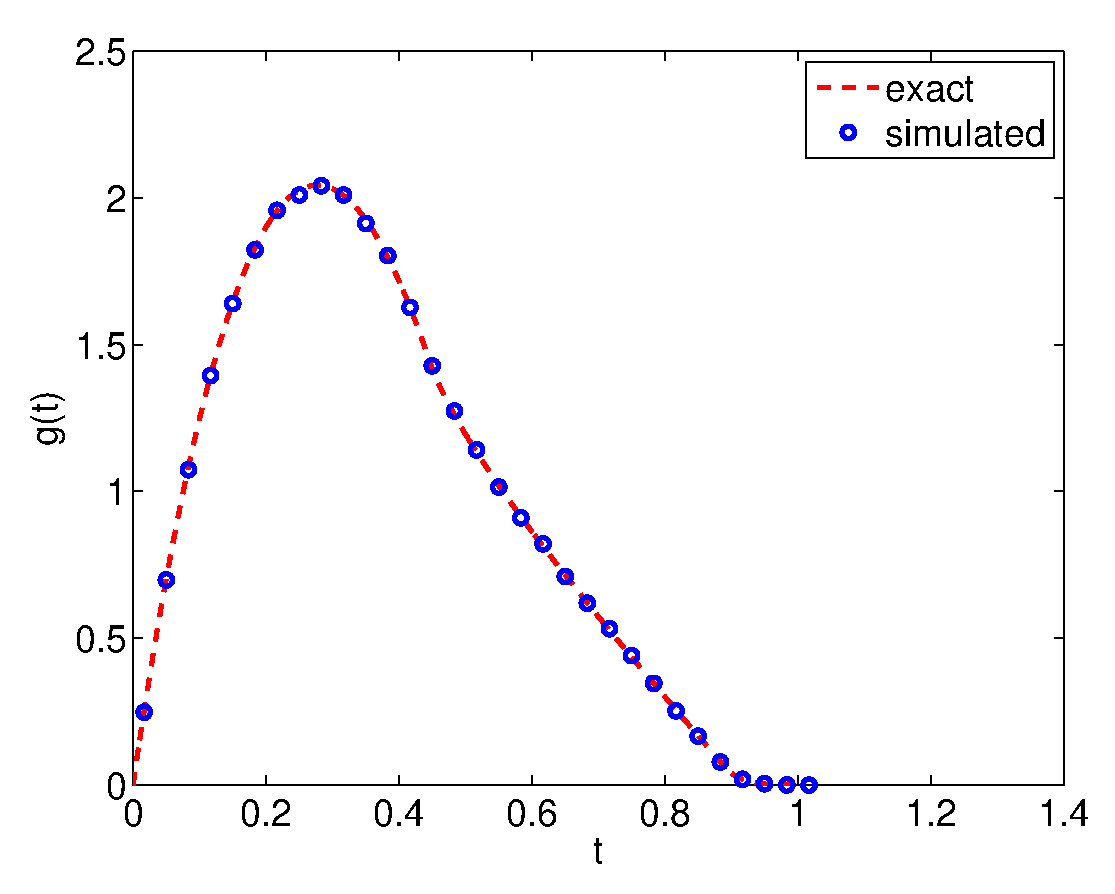
\includegraphics[width=0.24\columnwidth]{../Matlab/Plots/LinePicking_test_sim_rect.eps}}

        \subfloat[rectangle Manhattan (1:2)]{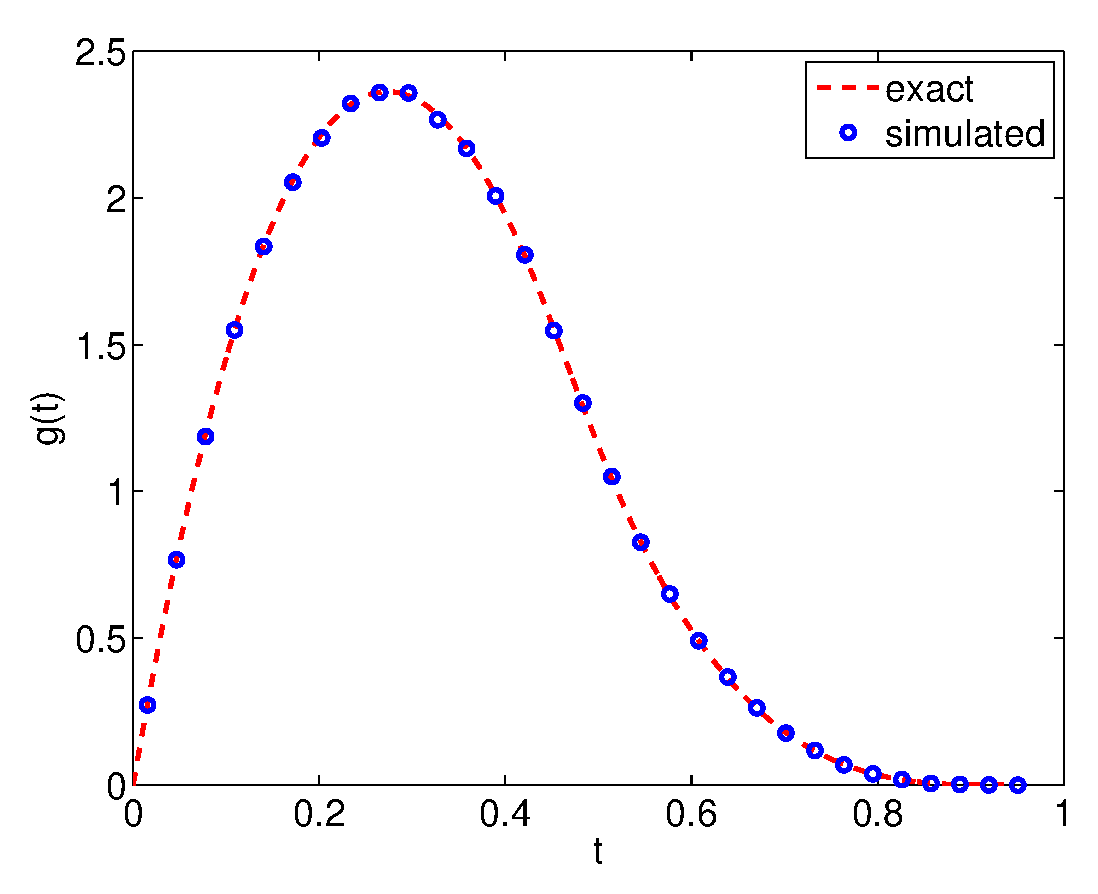
\includegraphics[width=0.24\columnwidth]{../Matlab/Plots/LinePicking_test_sim_rect_manhattan.eps}}
        \subfloat[rectangle max (1:2)]{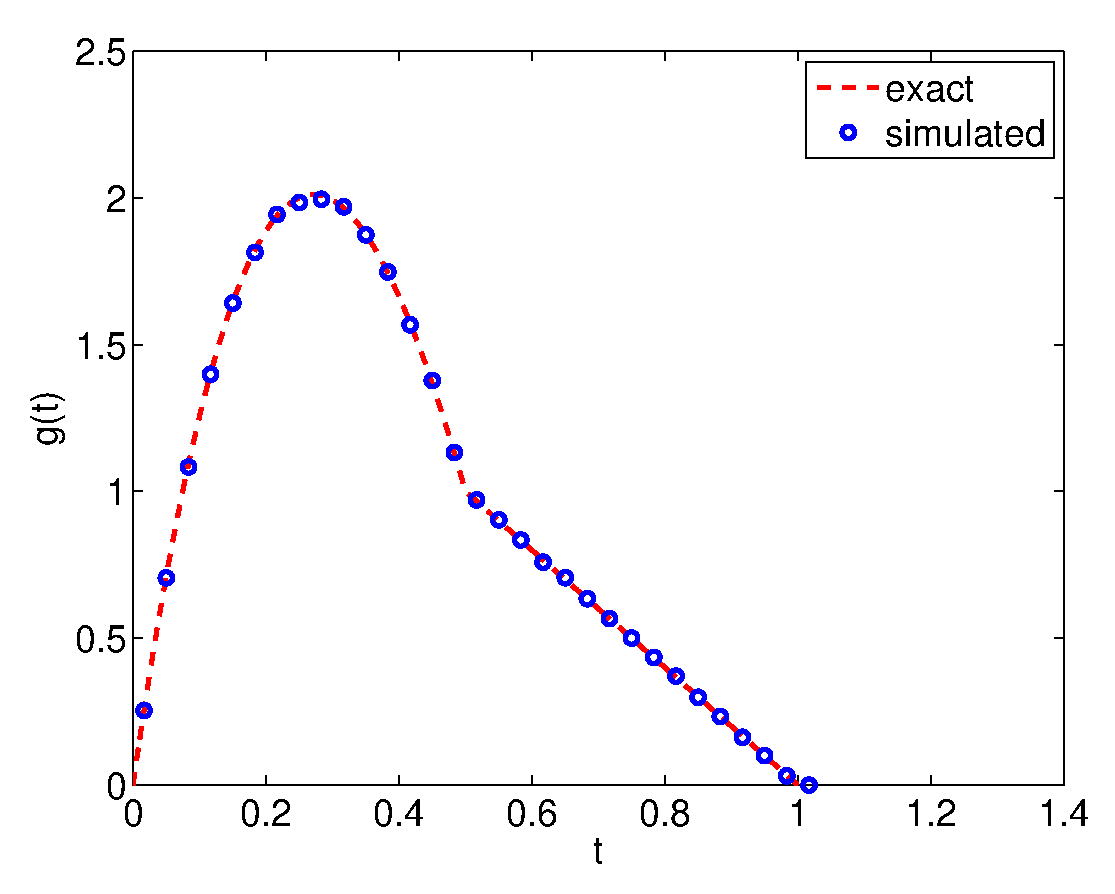
\includegraphics[width=0.24\columnwidth]{../Matlab/Plots/LinePicking_test_sim_rectangle_max.eps}}
        \subfloat[disk (2-ball)]{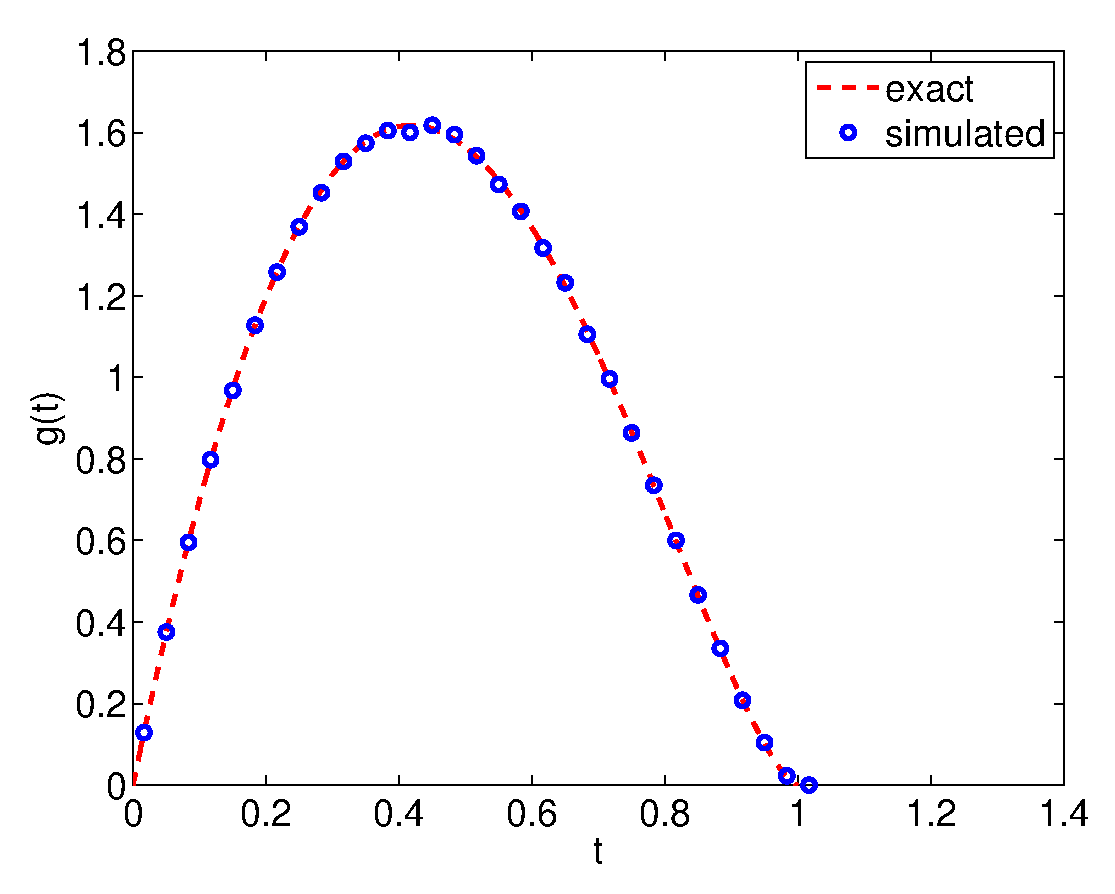
\includegraphics[width=0.24\columnwidth]{../Matlab/Plots/LinePicking_test_sim_disk.eps}}
        \subfloat[3-ball]{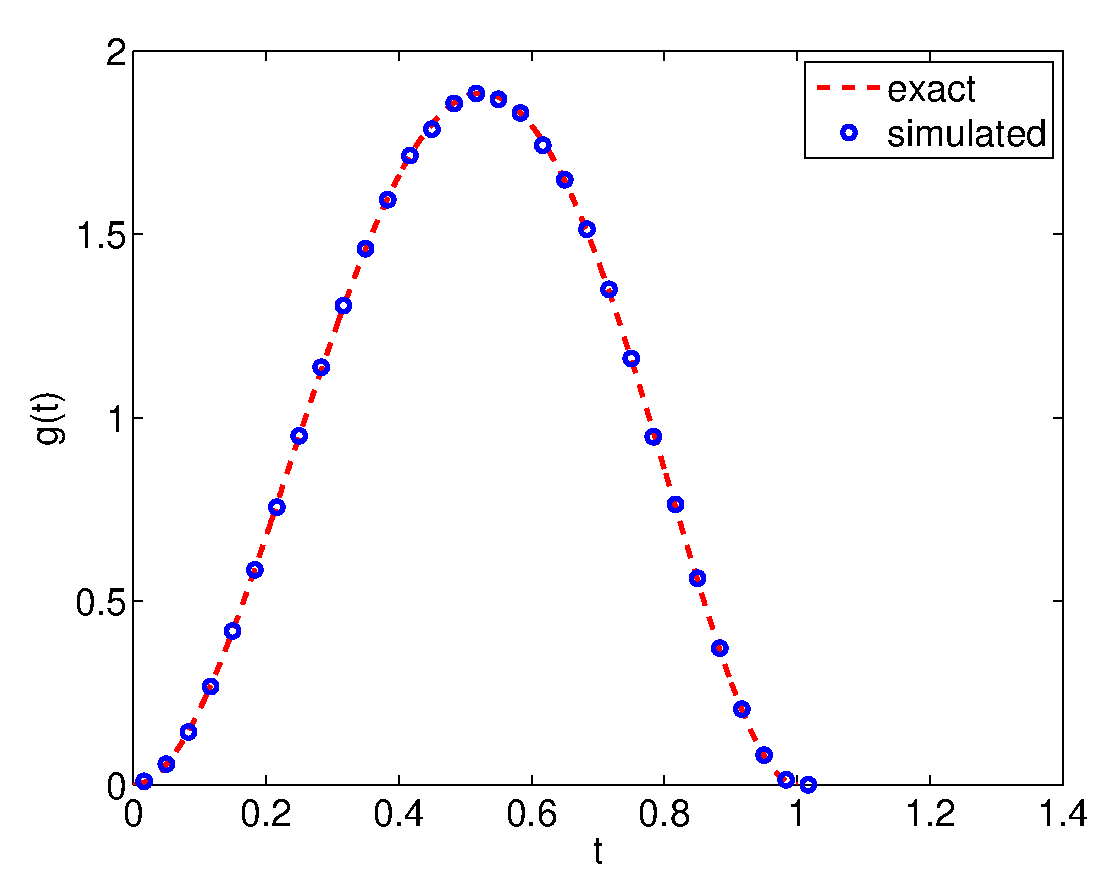
\includegraphics[width=0.24\columnwidth]{../Matlab/Plots/LinePicking_test_sim_3ball.eps}}

        \subfloat[4-ball]{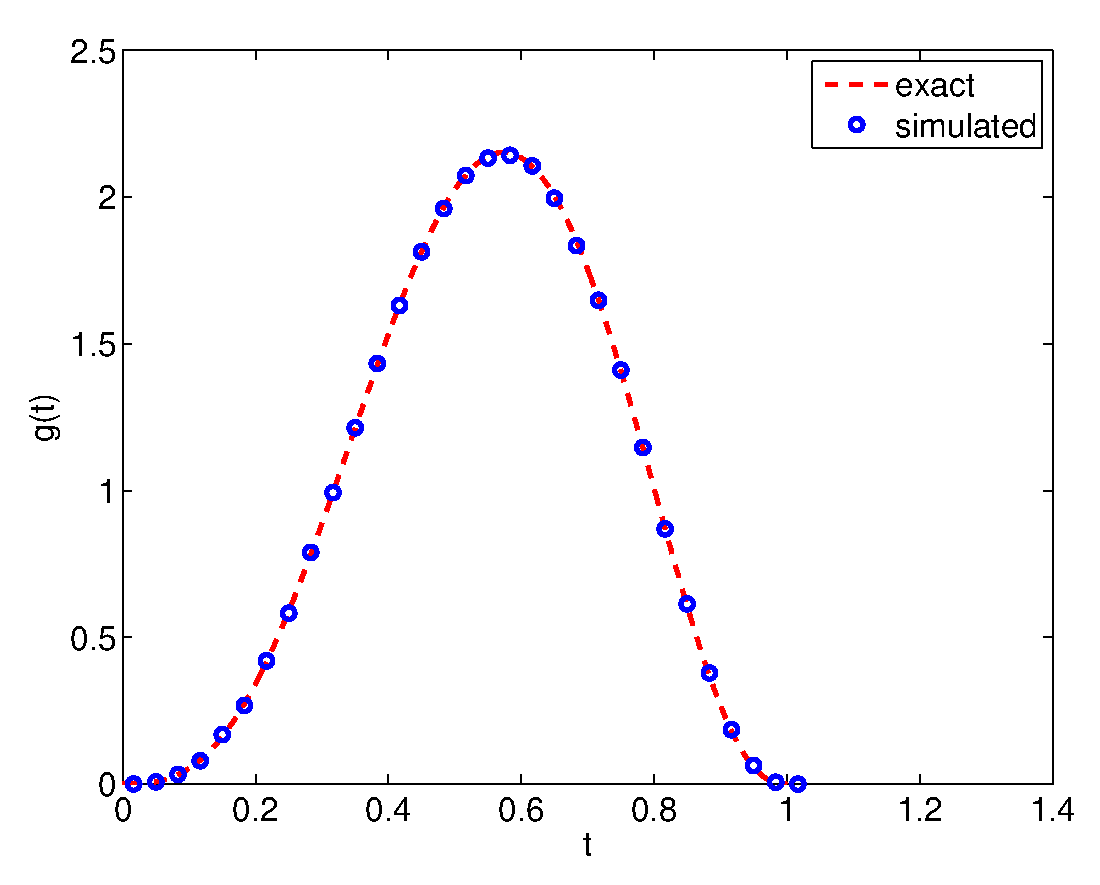
\includegraphics[width=0.24\columnwidth]{../Matlab/Plots/LinePicking_test_sim_4ball.eps}}
        \subfloat[circle (1-sphere)]{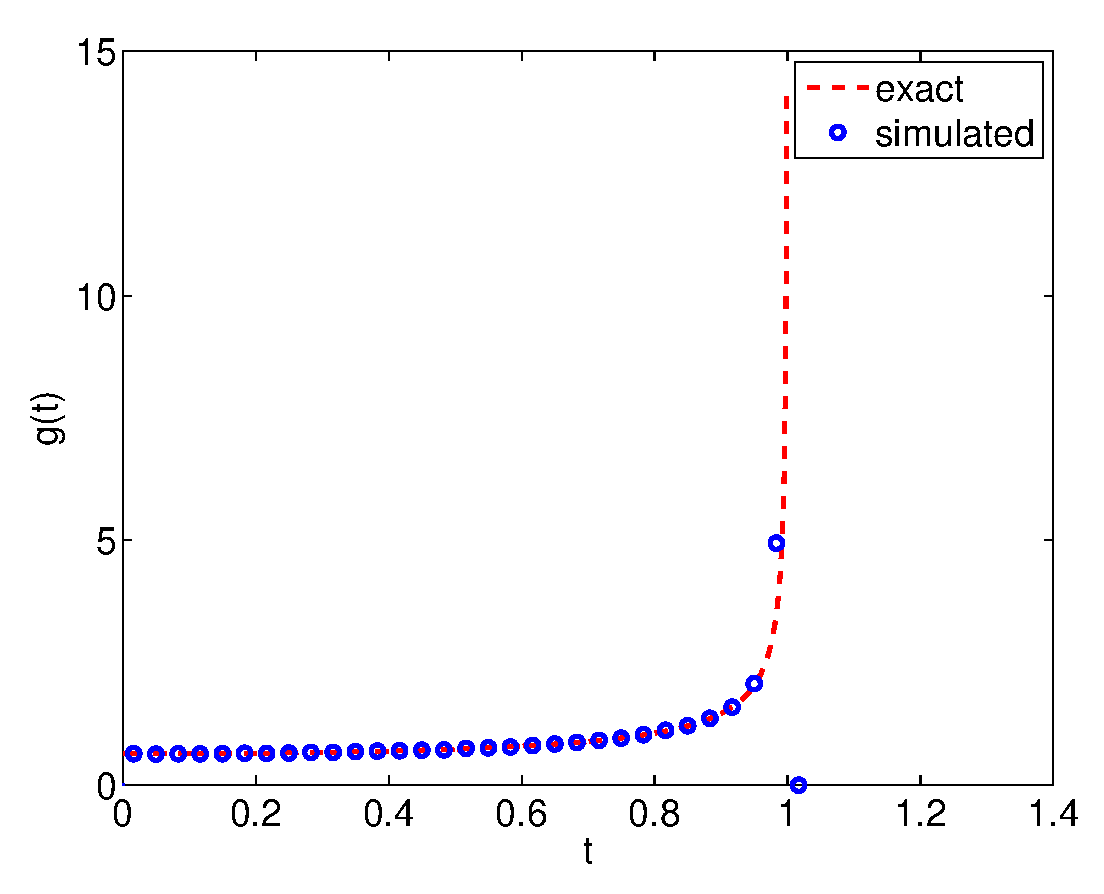
\includegraphics[width=0.24\columnwidth]{../Matlab/Plots/LinePicking_test_sim_circle.eps}}
        \subfloat[2-sphere]{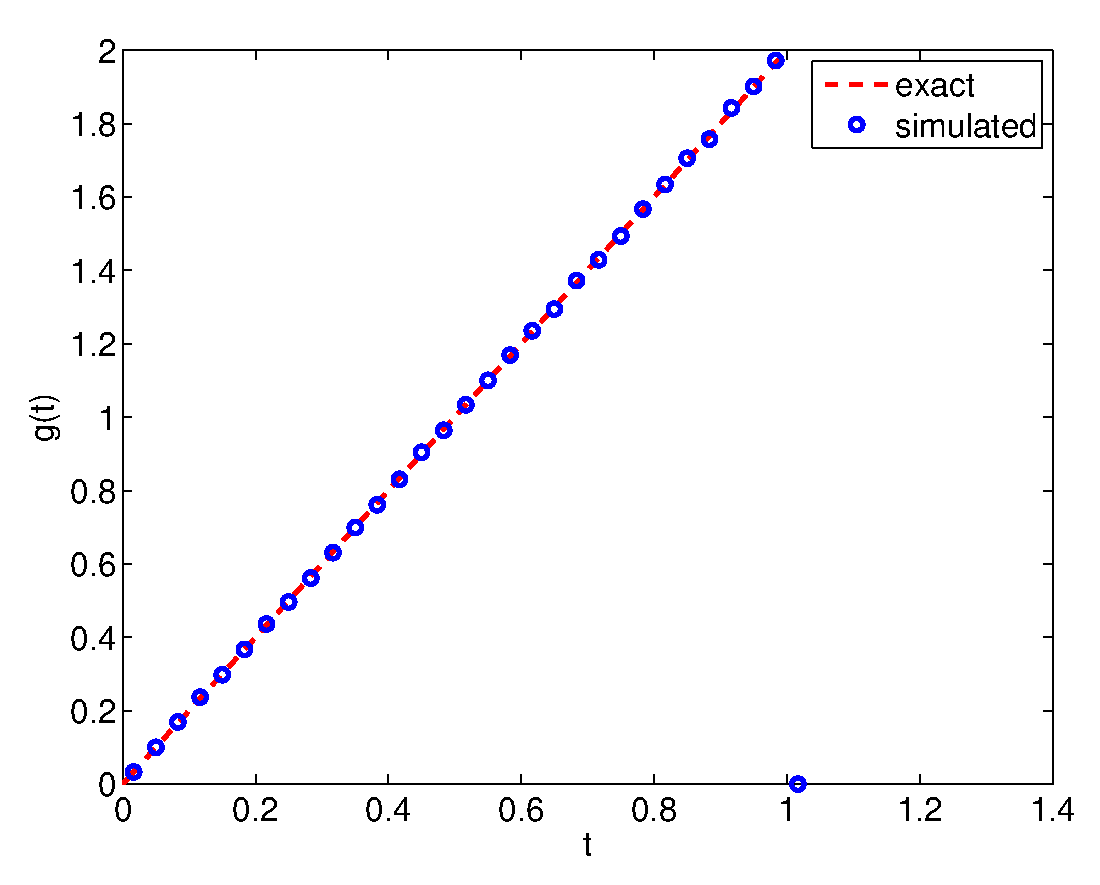
\includegraphics[width=0.24\columnwidth]{../Matlab/Plots/LinePicking_test_sim_2-sphere.eps}}
        \subfloat[3-sphere]{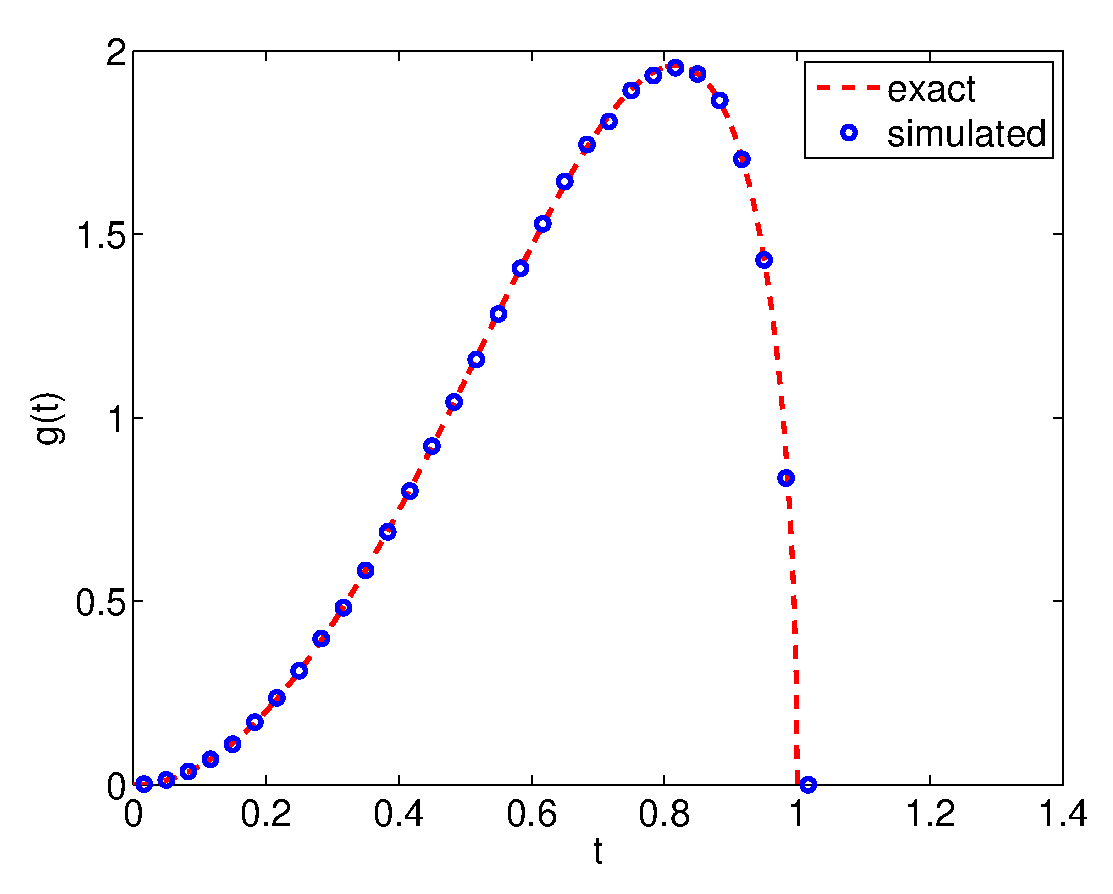
\includegraphics[width=0.24\columnwidth]{../Matlab/Plots/LinePicking_test_sim_3sphere.eps}}

        \subfloat[circle geodesic]{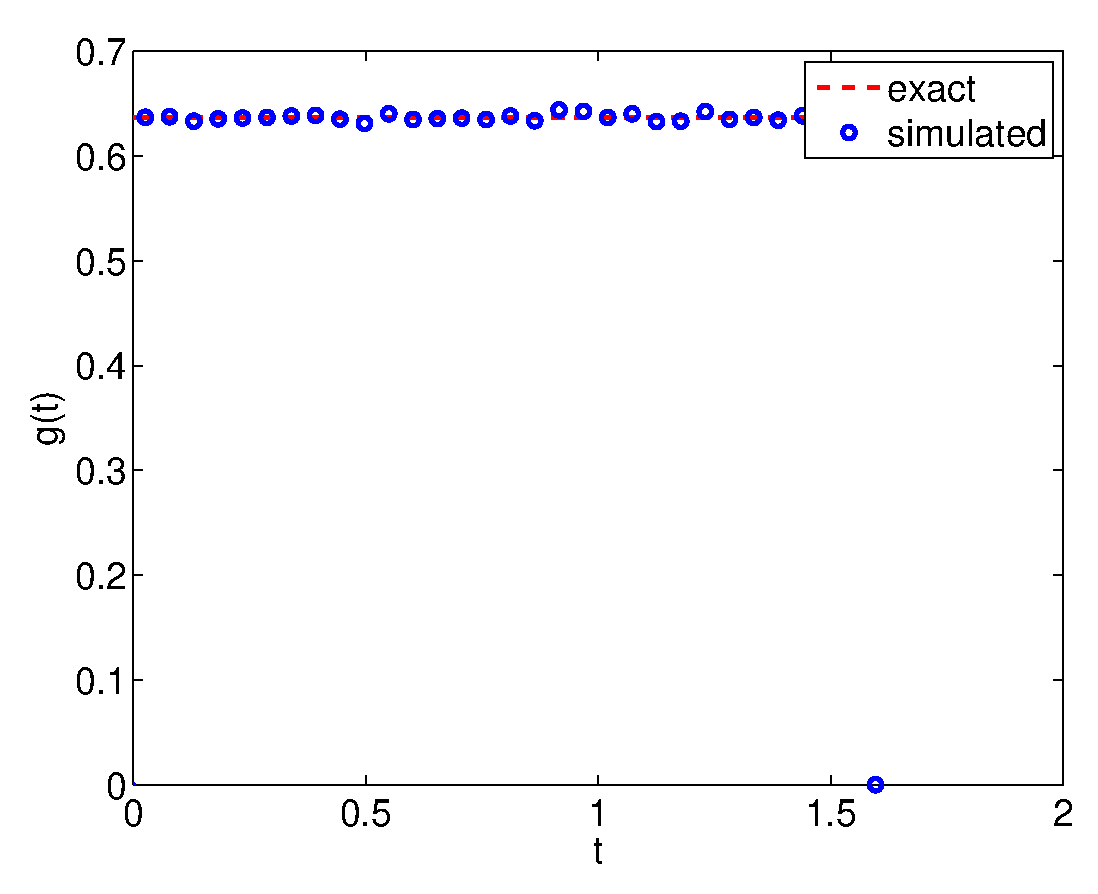
\includegraphics[width=0.24\columnwidth]{../Matlab/Plots/LinePicking_test_sim_circle_geodesic.eps}}
        \subfloat[sphere geodesic]{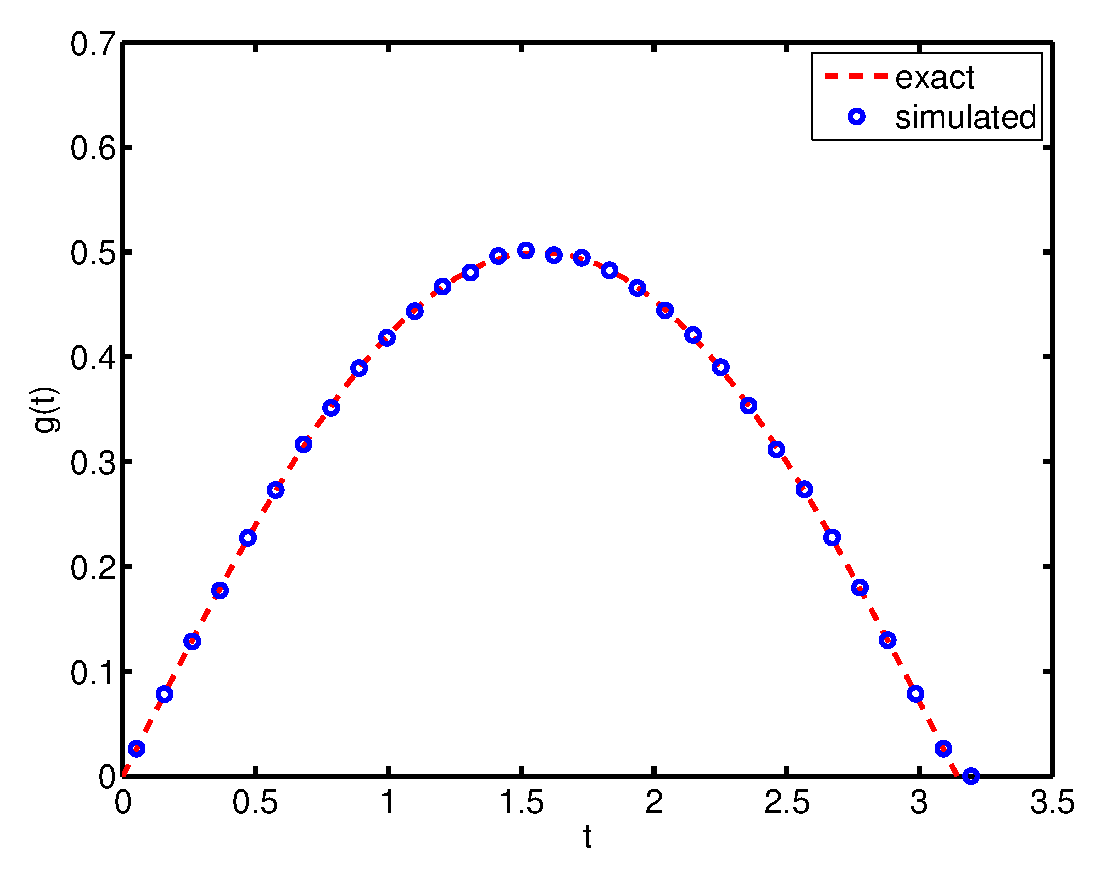
\includegraphics[width=0.24\columnwidth]{../Matlab/Plots/LinePicking_test_sim_sphere_geodesic.eps}}
        \subfloat[3-sphere geodesic]{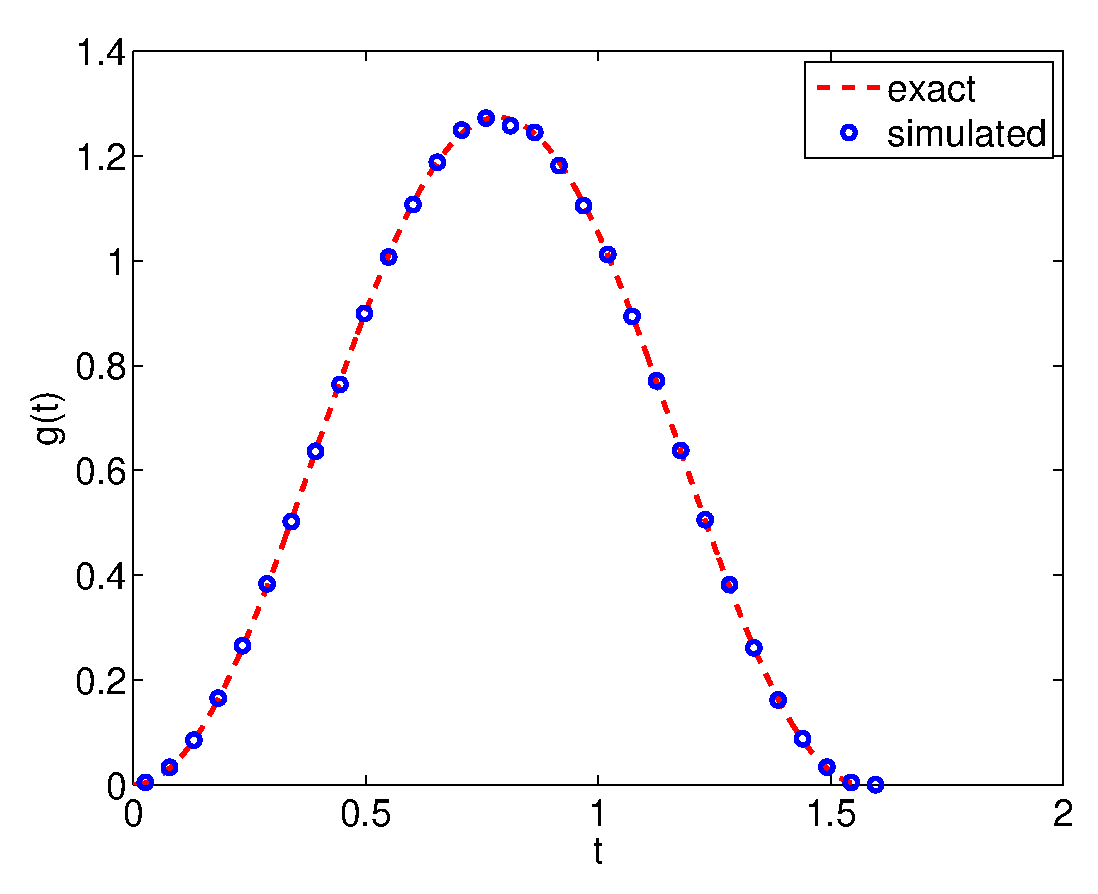
\includegraphics[width=0.24\columnwidth]{../Matlab/Plots/LinePicking_test_sim_3sphere_geodesic.eps}}
        \subfloat[prism geodesic]{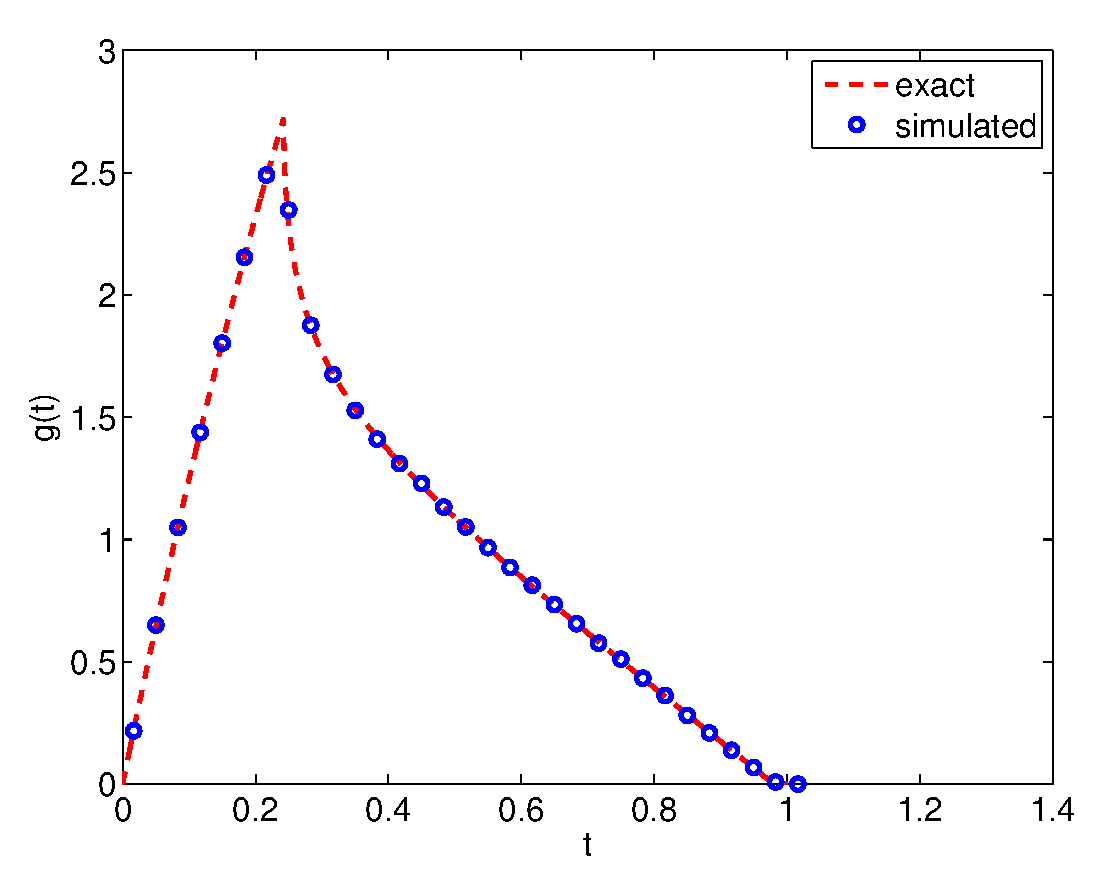
\includegraphics[width=0.24\columnwidth]{../Matlab/Plots/LinePicking_test_sim_prism_geodesic.eps}}

        \subfloat[cylindrical surface]{\includegraphics[width=0.24\columnwidth]{../Matlab/Plots/LinePicking_test_sim_cylindrical surface.eps}}
        \subfloat[cylindrical surface geodesic]{\includegraphics[width=0.24\columnwidth]{../Matlab/Plots/LinePicking_test_sim_cylindrical surface geodesic.eps}}
    \caption{\label{fig:sim_vs_exact}Comparisons of exactly calculated
      distributions and the distributions obtained by simulation. 
      1000000 simulated lines were used to draw the estimated PDF,
      which are binned into 30 equally spaced bins.}
  \end{center} 
\vspace{-4mm}
\end{figure}



\begin{table}[ht]
  \centering
  \begin{tabular}{r|rrrr}
                  problem &     mean & estimated mean & variance &  estimated var \\
     \hline 
                     line &   0.3333 &         0.3332 &   0.0556 &         0.0556 \\
                   square &   0.3687 &         0.3689 &   0.0307 &         0.0307 \\
                     cube &   0.3820 &         0.3820 &   0.0207 &         0.0207 \\
          rectangle (1:2) &   0.3599 &         0.3601 &   0.0371 &         0.0371 \\
rectangle Manhattan (1:2) &   0.3333 &         0.3335 &   0.0309 &         0.0308 \\
      rectangle max (1:2) &   0.3667 &         0.3711 &   0.0437 &         0.0437 \\
            disk (2-ball) &   0.4527 &         0.4529 &   0.0451 &         0.0451 \\
                   3-ball &   0.5143 &         0.5146 &   0.0355 &         0.0355 \\
                   4-ball &   0.5519 &         0.5521 &   0.0288 &         0.0288 \\
        circle (1-sphere) &   0.6366 &         0.6368 &   0.0947 &         0.0947 \\
                 2-sphere &   0.6667 &         0.6669 &   0.0556 &         0.0556 \\
                 3-sphere &   0.6791 &         0.6790 &   0.0389 &         0.0389 \\
          circle geodesic &   0.7854 &         0.7856 &   0.2056 &         0.2055 \\
          sphere geodesic &   0.7854 &         0.7857 &   0.1169 &         0.1170 \\
        3-sphere geodesic &   0.7854 &         0.7854 &   0.0806 &         0.0807 \\
           prism geodesic &   0.3645 &         0.3645 &   0.0436 &         0.0437 \\
      cylindrical surface &  -1.0000 &         0.4479 &  -1.0000 &         0.0327 \\
cylindrical surface geodesic &   0.4426 &         0.4426 &  -1.0000 &         0.0344 \\
  \end{tabular}
  \caption{Means and variances calculated exactly, and approximated by simulation.}
  \label{tab:mean_var_estimates}
\end{table}






\begin{table}[ht]
  \centering
  \begin{tabular}{r|r}
                  problem & PDF integral \\
     \hline 
                     line & 1.0000000000 \\
                   square & 1.0000000239 \\
                     cube & 1.0000000239 \\
          rectangle (1:2) & 0.9999999844 \\
rectangle Manhattan (1:2) & 0.9999999887 \\
      rectangle max (1:2) & 1.0000000000 \\
            disk (2-ball) & 1.0000000000 \\
                   3-ball & 1.0000000007 \\
                   4-ball & 1.0000000021 \\
        circle (1-sphere) & 1.0000000000 \\
                 2-sphere & 1.0000000000 \\
                 3-sphere & 1.0000000000 \\
          circle geodesic & 1.0000000000 \\
          sphere geodesic & 1.0000000000 \\
        3-sphere geodesic & 1.0000000000 \\
           prism geodesic & 0.9999999249 \\
      cylindrical surface & 0.9999977978 \\
cylindrical surface geodesic & 0.9999996398 \\
  \end{tabular}
  \caption{Numerically integrated PDFs (integrated using Matlab's {\tt quadgk} function)}
  \label{tab:numerical_pdf_sum}
\end{table}
